
\section{Distância entre os pontos}
\label{ssub:distância_entre_os_pontos}

Segundo \citeonline{cole1998}, para clusterizar termos de acordo com sua similaridade, deve-se definir uma medida de quão próximos dois termos estão. Uma medida de distância (métrica) deve ser definida de tal forma que:

\begin{itemize}
  \item Seja sempre positiva.
  \item Seja simétrica: a distância de um termo \(A_{i}\) para um termo \(A_{j}\) deve ser a mesma de \(A_{j}\) para \(A_{i}\).
  \item Seja reflexiva: se a distância entre \(A_{i}\) e \(A_{j}\) é zero, então \(A_{i} = A_{j}\).
  \item Respeite a desigualdade triangular: considerando os termos (\(A_{i}, A_{j}\) e \(A_k\)), a distância \(d(A_{i}, A_k)\) deve ser menor ou igual à soma das distâncias \(d(A_{i}, A_{j})\) e \(d(A_{j}, A_k)\)
\end{itemize}

Existem várias medidas de distância. Começamos pela distância Euclidiana entre dois pontos, \(A=(a_1, a_2, a_3, \ldots, a_n) \) e \(B=(b_1, b_2, b_3, \ldots, b_n) \), dada pela equação
%
\begin{align}
  dist(A, B) &= \sqrt{\displaystyle\sum_{i=1}^{n} (a_i-b_i)^2} \label{eq:euclidean}
\end{align}

Já a distância de Manhattan entre dois pontos, \(A=(a_1, a_2, a_3, \ldots, a_n) \) e \(B=(b_1, b_2, b_3, \ldots, b_n) \), é dada pela soma das diferenças absolutas de suas coordenadas:

\begin{align}
  dist(A, B) &= \displaystyle\sum_{i=1}^{n} |a_i-b_i| \label{eq:manhattan}
\end{align}

Em ambos os casos, temos que a distância entre do ponto A ao ponto B é a mesma distância do ponto B ao ponto A.

\begin{figure}[h]
  \centering
  \begin{subfigure}{.5\textwidth}
    \centering
    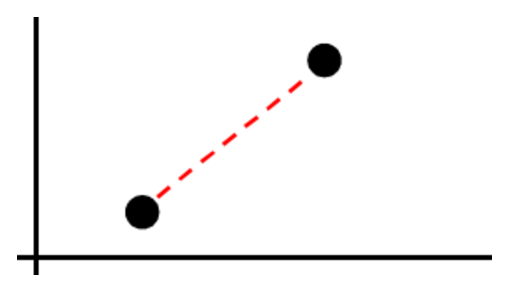
\includegraphics[scale=0.5]{figuras/euclidean.eps}
    \caption{Distância Euclidiana}
  \end{subfigure}%
  \begin{subfigure}{.5\textwidth}
    \centering
    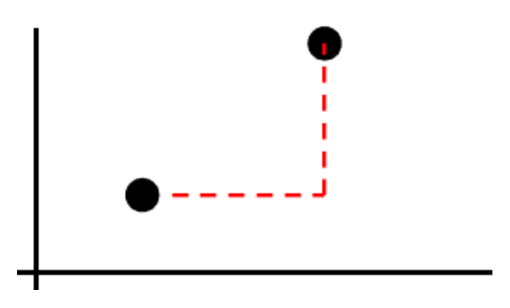
\includegraphics[scale=0.5]{figuras/manhattan.eps}
    \caption{Distância de Manhattan}
  \end{subfigure}
  \caption{Comparação entre distância Euclidiana e de Manhattan}
\end{figure}

Cada métrica pode gerar resultados diferentes no algoritmo \textit{k-means} e normalmente podem ser interpretadas do ponto de vista estatístico como uma escolha do modelo que gerou cada \textit{cluster}. A distância euclidiana pode ser associada a um modelo Gaussiano para gerar os pontos observados onde a média corresponde ao centróide de cada \textit{cluster} e o desvio padrão é o mesmo para todos os grupos.
